\documentclass[../Main.tex]{subfiles}
\begin{document}
  \chapter{2020-2021学年微积分（一）（下）期中考试}

  \section{基本计算题(每小题 6 分，共 60 分)}
  \begin{enumerate}
    \item 求$xy'-y=x^{2}\cos x$的通解.
      \vspace{12em}

    \item 求微分方程$y''-xy'^{2}=0$满足初始条件$y(0)=1$，$y'(0)=-2$的特解.
      \vspace{12em}

    \item 计算顶点为$A(1,1,1)$，$B(2,2,2)$，$C(1,2,2)$，$D(0,1,2)$的四面体$ABCD$的体积.
      \vspace{12em}

    \item 设函数$f$有二阶连续偏导数，$z=yf\left(x,x^{2} y\right)$，计算混合偏导$z
      _{xy}$.
      \vspace{13em}

    \item 设$w=x^{2} y z$，$z=x^{2}+y^{2}$，$x+y+z=4$，求$x=1$，$y=1$时导数$\frac{\mathrm{d}w}{\mathrm{d}x}$的值.
      \vspace{13em}

    \item 求$u=x^{2}+2y^{2}+3z^{2}$在$(1,1,1)$处沿曲面$x^{2}+y^{2}+z^{2}=3$的外法线方向的方向导数.
      \vspace{13em}

    \item 交换二次积分$I=\int_{0}^{1}\mathrm{d}y\int_{1-y}^{1+y^2}f(x,y)\mathrm{d}
      x$的积分次序.
      \vspace{13em}

    \item 计算$I=\iiint\limits_{\Omega}(x+2y+3z)\mathrm{d}x\mathrm{d}y\mathrm{d}z$，其中$\Omega$是由平面$x
      +y+z=1$与三个坐标面所围成的空间区域.
      \vspace{12em}

    \item 计算$I=\iiint\limits_{\Omega}\sqrt{x^{2}+y^{2}+z^{2}}\mathrm{d}x\mathrm{d}
      y\mathrm{d}z$，其中$\Omega$是由曲面$z=\sqrt{x^{2}+y^{2}}$与$z=1$所围成的区域.
      \vspace{12em}

    \item 求锥面$z=\sqrt{x^{2}+y^{2}}$被柱面$z^{2}=2x$所割下部分的面积$S$.
      \vspace{12em}
  \end{enumerate}

  \section{综合题(每小题 8 分，共 40 分)}
  \begin{enumerate}
    \item[11.] 设$f(x)$为连续函数，且满足积分方程$f(x)=\mathrm{e}^{x}-\int_{0}^{x}
      (x-t)f(t)\mathrm{d}t$，试求$f(x)$.
      \vspace{12em}

    \item[12.] 设$S$是曲线$L:
      \begin{cases}
        z=1-x^{2}, \\
        y=0
      \end{cases}$绕$z$轴的旋转曲面，求$S$的切平面，使其与已知平面$x+y+z=1$平行.
      \vspace{12em}

    \item[13.] 已知曲线$C:
      \begin{cases}
        x^{2}+2y^{2}-z=6, \\
        4x+2y+z=30
      \end{cases}$，求$C$上的点到$xOy$坐标面的距离的最大值.
      \vspace{12em}

    \item[14.] 计算$I=\iint\limits_{D}\left(y\mathrm{e}^{x}+\sqrt{x^{2}+y^{2}}\right
      )\mathrm{d}x\mathrm{d}y$，其中$D$是由心形线$r=a\left(1+\cos\theta\right)(a>
      0)$围成的区域.
      \vspace{12em}

    \item[15.] 讨论$f(x,y)=\sqrt{|xy|}$在点$(0,0)$处的连续性、偏导数存在性与可微性.
      \vspace{12em}
  \end{enumerate}

  \chapter{2020-2021学年微积分（一）（下）期中考试参考答案}
  \section{基本计算题(每小题 6 分，共 60 分)}
  \begin{enumerate}
    \item \textbf{Solution}. 方程变形为$y'-\frac{1}{x}y=x\cos x$，

      由一阶非齐次线性微分方程的通解公式得
      \[
        \begin{aligned}
          y = & \mathrm{e}^{-\int\left(-\frac{1}{x}\right)\mathrm{d}x}\left(C+\int\left(x\cos x\right)\mathrm{e}^{\int\left(-\frac{1}{x}\right)\mathrm{d}x}\mathrm{d}x\right) \\
          =   & x\left[C+\int\left(x\cos x\right)\cdot\frac{1}{x}\mathrm{d}x\right] = x\left(C+\int\cos x\mathrm{d}x\right) = x(C+\sin x)                                     \\
          =   & Cx+x\sin x.
        \end{aligned}
      \]

    \item \textbf{Solution}. 令$y'=p$，则方程变形为$p'-xp^{2}=0$，分离变量，得$\frac{\mathrm{d}p}{p^{2}}
      =x\mathrm{d}x$.

      两边积分，得$\int\frac{\mathrm{d}p}{p^{2}}=-\frac{1}{p}=\int x\mathrm{d}x=\frac{x^{2}}{2}
      +C_{1}$.

      将$y'(0)=p(0)=-2$代入上式，得$\frac{1}{2}=C_{1}$，所以$p=-\frac{1}{\frac{x^{2}}{2}+\frac{1}{2}}
      =-\frac{2}{x^{2}+1}$.

      因此$\int p \mathrm{d}x =y = \int -\frac{2}{x^{2}+1}\mathrm{d}x = -2\arctan
      x + C_{2}$.

      将$y(0)=1$代入上式，得$C_{2}=1$，所以特解为$y=-2\arctan x + 1$.

    \item \textbf{Solution}. $\overrightarrow{AB}= (1,1,1)$，$\overrightarrow{AC}
      = (0,1,1)$，$\overrightarrow{AD}= (-1,0,1)$，故

      $V=\frac{1}{6}\left|\left(\overrightarrow{AB}\times\overrightarrow{AC}\right
      )\cdot \overrightarrow{AD}\right| = \frac{1}{6}\left|
      \begin{vmatrix}
        1  & 1 & 1 \\
        0  & 1 & 1 \\
        -1 & 0 & 1
      \end{vmatrix}\right| = \frac{1}{6}.$

    \item \textbf{Solution}. $z_{x} = y\left(f_{1}+f_{2}\cdot 2xy\right)=y\left(f
      _{1}+2x y f_{2}\right)$，

      $z_{xy}= f_{1}+2xy f_{2} + y\left[x^{2}f_{12}+2x\left(f_{2}+yf_{22}\cdot x^{2}
      \right)\right] = f_{1}+4xyf_{2} + x^{2}y f_{12}+ 2x^{3} y^{2} f_{22}$.

    \item \textbf{Solution}. 设$F(x,y,z) = x^{2}+y^{2}-z$，$G(x,y,z)=x+y+z-4$.

      因$\frac{\partial (F,G)}{\partial (y,z)}\bigg|_{\left((1,1,2)\right)}=
      \begin{vmatrix}
        2y & -1 \\
        1  & 1
      \end{vmatrix}_{\left((1,1,2)\right)}=\left.(2y+1)\right|_{\left(1,1,2\right)}
      =3\neq 0$，

      所以方程组$\begin{cases}
        F(x,y,z)=0, \\
        G(x,y,z)=0
      \end{cases}$可以唯一确定两个具有连续导数的隐函数$y=y(x),z=z(x)$.

      方程组$\begin{cases}
        F(x,y,z) = x^{2}+y^{2}-z=0, \\
        G(x,y,z)=x+y+z-4=0
      \end{cases}$两边对$x$求导，得 $\begin{cases}
        2x+2y\frac{\mathrm{d}y}{\mathrm{d}x}-\frac{\mathrm{d}z}{\mathrm{d}x}=0, \\[6pt]
        1+\frac{\mathrm{d}y}{\mathrm{d}x}+\frac{\mathrm{d}z}{\mathrm{d}x}=0.
      \end{cases}$

      将$x=1$，$y=1$代入上式，得$\begin{cases}
        2\frac{\mathrm{d}y}{\mathrm{d}x}-\frac{\mathrm{d}z}{\mathrm{d}x}=-2, \\[6pt]
        \frac{\mathrm{d}y}{\mathrm{d}x}+\frac{\mathrm{d}z}{\mathrm{d}x}=-1
      \end{cases}$，解得$\begin{cases}
        \frac{\mathrm{d}y}{\mathrm{d}x}= -1, \\[6pt]
        \frac{\mathrm{d}z}{\mathrm{d}x}= 0.
      \end{cases}$

      所以$\frac{\mathrm{d}w}{\mathrm{d}x}= 2xyz + x^{2} z \cdot \frac{\mathrm{d}y}{\mathrm{d}x}
      + x^{2} y \cdot \frac{\mathrm{d}z}{\mathrm{d}x}= 4+2\frac{\mathrm{d}y}{\mathrm{d}x}
      +\frac{\mathrm{d}z}{\mathrm{d}x}= 2$.

    \item \textbf{Solution}. 设$F(x,y,z) = x^{2}+y^{2}+z^{2}-3$，则$\nabla F = (2
      x,2y,2z)$，

      故可以取曲面$F(x,y,z)=0$在$(1,1,1)$处的单位外法线$\boldsymbol{n}= \frac{1}{\sqrt{3}}
      (1,1,1)$.

      又$\nabla u|_{(1,1,1)}= (2x,4y,6z)|_{(1,1,1)}= (2,4,6)$，

      所以$u$在$(1,1,1)$处沿曲面$x^{2}+y^{2}+z^{2}=3$的外法线方向的方向导数$\frac{\partial
      u}{\partial \boldsymbol{n}}= \nabla u \cdot \boldsymbol{n}= 4\sqrt{3}$.

    \item \textbf{Solution}.

      \noindent
      \begin{minipage}[c]{0.6\textwidth}
        积分区域如图所示. 所以
        \[
          \begin{aligned}
            I = & \int_{0}^{1}\mathrm{d}y\int_{1-y}^{1+y^2}f(x,y)\mathrm{d}x                                                              \\
            =   & \iint\limits_{D_1}f(x,y)\mathrm{d}x\mathrm{d}y + \iint\limits_{D_2}f(x,y)\mathrm{d}x\mathrm{d}y                         \\
            =   & \int_{0}^{1}\mathrm{d}x\int_{1-x}^{1}f(x,y)\mathrm{d}y + \int_{1}^{2}\mathrm{d}x\int_{\sqrt{x-1}}^{1}f(x,y)\mathrm{d}y.
          \end{aligned}
        \]
      \end{minipage}
      \hfill %
      \begin{minipage}[c]{0.5\textwidth}
        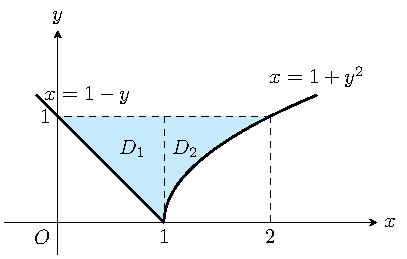
\includegraphics[width=6cm]{2021x-figure1.pdf} % 引入图片源
      \end{minipage}

    \item \textbf{Solution}.

      \textbf{法一}. $\Omega$是由平面$x+y+z=1$与三个坐标面所围成的四面体，其体积$V
      = \frac{1}{6}$，形心坐标为$\left(\frac{1}{4},\frac{1}{4},\frac{1}{4}\right)$.

      故$I = \iiint\limits_{\Omega}(x+2y+3z)\mathrm{d}v = \iiint\limits_{\Omega}x
      \mathrm{d}v + 2\iiint\limits_{\Omega}y\mathrm{d}v + 3\iiint\limits_{\Omega}
      z\mathrm{d}v = (1+2+3)\cdot \frac{1}{4}V = \frac{1}{4}$.

      \textbf{法二}. 令$\begin{cases}
        u = x+y+z,             \\
        v = \frac{y+z}{x+y+z}, \\
        w = \frac{z}{y+z}
      \end{cases}$，则$\begin{cases}
        x = u(1-v),  \\
        y = uv(1-w), \\
        z = uvw
      \end{cases}$，$|J| = \left|
      \begin{vmatrix}
        1-v    & -u     & 0   \\
        v(1-w) & u(1-w) & -uv \\
        vw     & uv     & uv
      \end{vmatrix}\right| = u^{2} v$.

      积分区域$\Omega$在$uvw$坐标系中的表示为$0\leq u \leq 1$，$0\leq v \leq 1$，$0
      \leq w \leq 1$，所以
      \[
        \begin{aligned}
          I = & \iiint\limits_{\Omega}(x+2y+3z)\mathrm{d}x\mathrm{d}y\mathrm{d}z = \int_{0}^{1}\mathrm{d}u\int_{0}^{1}\mathrm{d}v\int_{0}^{1}\left[u(1-v)+2uv(1-w)+3uvw\right]u^{2} v\mathrm{d}w \\
          =   & \int_{0}^{1}u^{3}\mathrm{d}u\int_{0}^{1}v\mathrm{d}v\int_{0}^{1}\left(1+v+vw\right)\mathrm{d}w = \frac{1}{4}\int_{0}^{1}v\left(1+v+\frac{v}{2}\right)\mathrm{d}v = \frac{1}{4}.
        \end{aligned}
      \]

      此代换考虑比例关系，先确定总量$u=x+y+z$，再确定后两项$y+z$占总量的比例$v$，最后确定$z$占后两项的总和$y
      +z$的比例$w$，从而把积分限转化为常数.

      再考虑一例：计算$I=\iint\limits_{D}x^{2} y\mathrm{d}x\mathrm{d}y$，其中$D$是以$(
      0,0)$，$(3,0)$，$(0,4)$为顶点的三角形及其内部.

      \textbf{Solution}. 斜边的方程为$4x+3y = 12$，即$\frac{1}{3}x+\frac{1}{4}y=1$，令$\begin{cases}
        u = \frac{1}{3}x+\frac{1}{4}y,                     \\
        v = \frac{\frac{1}{4}y}{\frac{1}{3}x+\frac{1}{4}y}
      \end{cases}$，

      则$\begin{cases}
        x = 3u(1-v), \\
        y = 4uv
      \end{cases}$，$|J| = \left|
      \begin{vmatrix}
        3(1-v) & -3u \\
        4v     & 4u
      \end{vmatrix}\right| = 12u$. 故
      \[
        \begin{aligned}
          I = & \iint\limits_{D}x^{2} y\mathrm{d}x\mathrm{d}y = \int_{0}^{1}\mathrm{d}u\int_{0}^{1}\left[3u(1-v)\right]^{2} \cdot 4uv \cdot 12u\mathrm{d}v \\
          =   & 432\int_{0}^{1}u^{4}\mathrm{d}u\int_{0}^{1}v(1-v)^{2}\mathrm{d}v = 432\cdot\frac{1}{5}\cdot\frac{2!}{4!}= \frac{36}{5}.
        \end{aligned}
      \]

    \item \textbf{Solution}. 用球坐标代换，锥面$z=\sqrt{x^{2}+y^{2}}$对应的球坐标方程为$\varphi
      = \frac{\pi}{4}(z\geq 0)$，所以
      \[
        \begin{aligned}
          I = & \iiint\limits_{\Omega}\sqrt{x^2+y^2+z^2}\mathrm{d}x\mathrm{d}y\mathrm{d}z = \int_{0}^{2\pi}\mathrm{d}\theta\int_{0}^{\frac{\pi}{4}}\mathrm{d}\varphi\int_{0}^{\frac{1}{\cos \varphi}}\rho^{3}\sin \varphi\mathrm{d}\rho \\
          =   & 2\pi\int_{0}^{\frac{\pi}{4}}\sin \varphi\mathrm{d}\varphi\int_{0}^{\frac{1}{\cos \varphi}}\rho^{3}\mathrm{d}\rho = \frac{\pi}{2}\int_{0}^{\frac{\pi}{4}}\frac{\sin \varphi}{\cos^{4} \varphi}\mathrm{d}\varphi          \\
          =   & -\frac{\pi}{2}\int_{0}^{\frac{\pi}{4}}\frac{1}{\cos^4 \varphi}\mathrm{d}(\cos \varphi) = \left.\frac{\pi}{2}\cdot \frac{1}{3\cos^{3} \varphi}\right|_{0}^{\frac{\pi}{4}}= \frac{\pi}{6}\left(2\sqrt{2}-1\right).
        \end{aligned}
      \]

    \item \textbf{Solution}. 联立$\begin{cases}
        z=\sqrt{x^2+y^2}, \\
        z^{2}=2x
      \end{cases}$，得锥面和柱面的交线满足$x^{2}+y^{2}=2x$，即$(x-1)^{2}+y^{2}=1$，

      在$xOy$平面上的投影为圆域$D=\{(x,y)|(x-1)^{2}+y^{2}\leq 1\}$，

      锥面上被柱面所割下的部分对应于$D$内的点. 所以
      \[
        \begin{aligned}
          S = & \iint\limits_{S}\mathrm{d}S = \iint\limits_{D}\sqrt{1+\left(\frac{\partial z}{\partial x}\right)^2+\left(\frac{\partial z}{\partial y}\right)^2}\mathrm{d}x\mathrm{d}y \\
          =   & \iint\limits_{D}\sqrt{1+\frac{x^2}{x^2+y^2}+\frac{y^2}{x^2+y^2}}\mathrm{d}x\mathrm{d}y = \sqrt{2}\iint\limits_{D}\mathrm{d}x\mathrm{d}y                                \\
          =   & \sqrt{2}\pi.
        \end{aligned}
      \]
  \end{enumerate}

  \section{综合题(每小题 8 分，共 40 分)}
  \begin{enumerate}
    \item[11.] \textbf{Solution}. 因为$f(x)$是连续函数，所以$\mathrm{e}^{x}-\int_{0}
      ^{x}(x-t)f(t)\mathrm{d}t$是可导的，从而$f(x)$也是可导的.

      对方程两边求导，得$f'(x) = \mathrm{e}^{x} - \int_{0}^{x}f(t)\mathrm{d}t$.同理可知$f
      '(x)$也是可导的，

      所以对方程两边再次求导，得$f''(x) = \mathrm{e}^{x} - f(x)$，即$f''(x)+f(x) =
      \mathrm{e}^{x}$.

      齐次方程$f''(x)+f(x)=0$的特征方程为$r^{2}+1=0$，解得$r=\pm i$，

      所以齐次方程的通解为$C_{1}\cos x + C_{2}\sin x$.

      对于$y=\mathrm{e}^{x}$，$\lambda = 1$不是齐次方程的特征根，所以可设非齐次方程的特解为$y
      ^{*} = A\mathrm{e}^{x}$，

      将其代入非齐次方程，得$2A\mathrm{e}^{x} = \mathrm{e}^{x}$，所以$A=\frac{1}{2}$.

      因此非齐次方程的通解为$f(x) = C_{1}\cos x + C_{2}\sin x + \frac{1}{2}\mathrm{e}
      ^{x}$.

      在方程$f(x)=\mathrm{e}^{x}-\int_{0}^{x}(x-t)f(t)\mathrm{d}t$中令$x=0$，得$f
      (0)=1$；

      在方程$f'(x) = \mathrm{e}^{x} - \int_{0}^{x}f(t)\mathrm{d}t$中令$x=0$，得$f
      '(0)=1$.

      将$f(0)=1$，$f'(0)=1$代入非齐次方程的通解，得$\begin{cases}
        C_{1} + \frac{1}{2}= 1, \\[6pt]
        C_{2} + \frac{1}{2}= 1
      \end{cases}$，解得$\begin{cases}
        C_{1} = \frac{1}{2}, \\[6pt]
        C_{2} = \frac{1}{2}.
      \end{cases}$

      因此$f(x) = \frac{1}{2}\cos x + \frac{1}{2}\sin x + \frac{1}{2}\mathrm{e}^{x}$.

    \item[12.] \textbf{Solution}. 由题可知旋转曲面的方程为$z=1-x^{2}-y^{2}$，令$F
      (x,y,z) = x^{2}+y^{2}+z-1$，

      则$\nabla F = (2x,2y,1)$. 令$\nabla F // (1,1,1)$，得$x=y=\frac{1}{2}$，

      代入方程可得$z=\frac{1}{2}$，所以切平面方程为$x-\frac{1}{2}+y-\frac{1}{2}+z
      -\frac{1}{2}=0$，即$2x + 2y + 2z = 3$.

    \item[13.] \textbf{Solution}. 即在约束条件$\begin{cases}
        x^{2}+2y^{2}-z=6, \\
        4x+2y+z=30
      \end{cases}$下，求$|z|$的最大值.

      用Lagrange乘数法，设$L(x,y,z,\lambda,\mu) = z^{2} + \lambda(x^{2}+2y^{2}-z-
      6) + \mu(4x+2y+z-30)$，则
      \[
        \begin{cases}
          \frac{\partial L}{\partial x}= 2\lambda x + 4\mu = 0,        \\[6pt]
          \frac{\partial L}{\partial y}= 4\lambda y + 2\mu = 0,        \\[6pt]
          \frac{\partial L}{\partial z}= 2z - \lambda + \mu = 0,       \\[6pt]
          \frac{\partial L}{\partial \lambda}= x^{2}+2y^{2}-z - 6 = 0, \\[6pt]
          \frac{\partial L}{\partial \mu}= 4x+2y+z-30 = 0.
        \end{cases}
      \]

      $\frac{\partial L}{\partial x}-2\frac{\partial L}{\partial y}$，得$2\lambda
      x = 8\lambda y$，所以$x=4y$或$\lambda=0$.

      若$\lambda=0$，则$\frac{\partial L}{\partial x}= 4\mu = 0$，$\frac{\partial
      L}{\partial z}= 2z = 0$，代入约束条件得$\begin{cases}
        x^{2}+2y^{2}=6, \\
        4x+2y=30
      \end{cases}$，此方程组无解.

      因此$x=4y$，故$\begin{cases}
        16y^{2}+2y^{2}-z=6, \\
        16y+2y+z=30
      \end{cases}$，解得$\begin{cases}
        y=-2, \\
        z=66.
      \end{cases}$或$\begin{cases}
        y=1,  \\
        z=12.
      \end{cases}$

      比较可知距离$xOy$平面的距离的最大值为$66$.

    \item[14.] \textbf{Solution}.

      \noindent
      \begin{minipage}[c]{0.6\textwidth}
        积分区域如图所示. 由对称性可知$\iint\limits_{D}y\mathrm{e}^{x}\mathrm{d}x
        \mathrm{d}y=0$，所以
        \[
          \begin{aligned}
            I = & \iint\limits_{D}\left(y\mathrm{e}^{x}+\sqrt{x^2+y^2}\right)\mathrm{d}x\mathrm{d}y                                                                                                     \\
            =   & 2 \iint\limits_{D_1}\sqrt{x^2+y^2}\mathrm{d}x\mathrm{d}y                                                                                                                              \\
            =   & 2\int_{0}^{\pi}\mathrm{d}\theta\int_{0}^{a\left(1+\cos \theta\right)}r^{2}\mathrm{d}r = \frac{2a^3}{3}\int_{0}^{\pi}\left(1+\cos \theta\right)^{3}\mathrm{d}\theta                    \\
            =   & \frac{2a^3}{3}\int_{0}^{\pi}\left(1+3\cos \theta + 3\cos^{2} \theta + \cos^{3} \theta\right)\mathrm{d}\theta                                                                          \\
            =   & \frac{2a^3}{3}\int_{0}^{\pi}\left(1+3\cos^{2} \theta\right)\mathrm{d}\theta = \frac{2\pi a^3}{3}+ 4a^{3}\int_{0}^{\frac{\pi}{2}}\cos^{2} \theta\mathrm{d}\theta = \frac{5\pi a^3}{3}.
          \end{aligned}
        \]
      \end{minipage}
      \hfill %
      \begin{minipage}[c]{0.5\textwidth}
        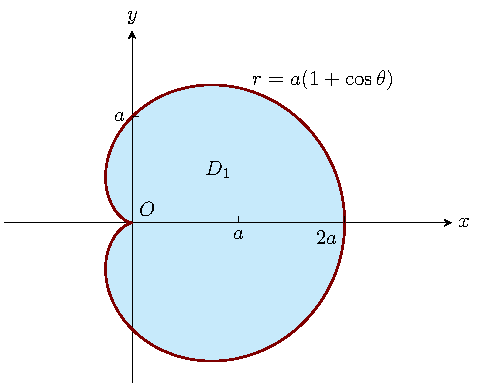
\includegraphics[width=6cm]{2021x-figure2.pdf} % 引入图片源
      \end{minipage}

    \item[15.] \textbf{Solution}. $\forall\,\varepsilon > 0$，取$\delta = \sqrt{2}
      \varepsilon$，则当$||(x,y)||= \sqrt{x^{2}+y^{2}}<\delta$时，有
      \[
        |f(x,y)-f(0,0)| = \sqrt{|xy|}\leq \sqrt{\frac{x^{2}+y^{2}}{2}}< \frac{\delta}{\sqrt{2}}
        = \varepsilon
      \]

      所以$\lim_{\substack{x\to 0 \\ y\to 0}}\sqrt{|xy|}=0=f(0,0)$，函数$f(x,y)$在原点处连续.

      又$f(x,0)=f(0,y)\equiv 0$，所以$f_{x}(0,0)=f_{y}(0,0)=0$，因此函数$f(x,y)$在原点处的偏导数存在.

      考察$\lim_{\substack{x\to 0 \\ y\to 0}}\frac{f(x,y)-f(0,0)-f_{x}(0,0)x-f_{y}(0,0)y}{\sqrt{x^{2}+y^{2}}}
      = \lim_{\substack{x\to 0 \\ y\to 0}}\sqrt{\frac{|xy|}{x^{2}+y^{2}}}$.

      当$y=x,x\to0,y\to0$时，$\lim_{\substack{x\to 0 \\ y\to 0}}\sqrt{\frac{|xy|}{x^{2}+y^{2}}}
      = \lim_{x\to0}\sqrt{\frac{|x^{2}|}{2x^{2}}}= \frac{1}{\sqrt{2}}$，所以$\lim
      _{\substack{x\to 0 \\ y\to 0}}\sqrt{\frac{|xy|}{x^{2}+y^{2}}}\neq 0$，

      因此函数$f(x,y)$在原点处不可微.
  \end{enumerate}
\end{document}
